\documentclass{article}

%%%%%%%%%%%%%%%%%%%%%%%%%%%%%%%%%%%%%%%%%
% Lachaise Assignment
% Structure Specification File
% Version 1.0 (26/6/2018)
%
% This template originates from:
% http://www.LaTeXTemplates.com
%
% Authors:
% Marion Lachaise & François Févotte
% Vel (vel@LaTeXTemplates.com)
%
% License:
% CC BY-NC-SA 3.0 (http://creativecommons.org/licenses/by-nc-sa/3.0/)
% 
%%%%%%%%%%%%%%%%%%%%%%%%%%%%%%%%%%%%%%%%%

%----------------------------------------------------------------------------------------
%	PACKAGES AND OTHER DOCUMENT CONFIGURATIONS
%----------------------------------------------------------------------------------------

\usepackage{amsmath,amsfonts,stmaryrd,amssymb} % Math packages

\usepackage{enumerate} % Custom item numbers for enumerations

\usepackage[ruled]{algorithm2e} % Algorithms

\usepackage[framemethod=tikz]{mdframed} % Allows defining custom boxed/framed environments

\usepackage{listings} % File listings, with syntax highlighting
\lstset{
	basicstyle=\ttfamily, % Typeset listings in monospace font
}

%----------------------------------------------------------------------------------------
%	DOCUMENT MARGINS
%----------------------------------------------------------------------------------------

\usepackage{geometry} % Required for adjusting page dimensions and margins

\geometry{
	paper=a4paper, % Paper size, change to letterpaper for US letter size
	top=2.5cm, % Top margin
	bottom=3cm, % Bottom margin
	left=2.5cm, % Left margin
	right=2.5cm, % Right margin
	headheight=14pt, % Header height
	footskip=1.5cm, % Space from the bottom margin to the baseline of the footer
	headsep=1.2cm, % Space from the top margin to the baseline of the header
	%showframe, % Uncomment to show how the type block is set on the page
}

%----------------------------------------------------------------------------------------
%	FONTS
%----------------------------------------------------------------------------------------

\usepackage[utf8]{inputenc} % Required for inputting international characters
\usepackage[T1]{fontenc} % Output font encoding for international characters

\usepackage{XCharter} % Use the XCharter fonts

%----------------------------------------------------------------------------------------
%	COMMAND LINE ENVIRONMENT
%----------------------------------------------------------------------------------------

% Usage:
% \begin{commandline}
%	\begin{verbatim}
%		$ ls
%		
%		Applications	Desktop	...
%	\end{verbatim}
% \end{commandline}

\mdfdefinestyle{commandline}{
	leftmargin=10pt,
	rightmargin=10pt,
	innerleftmargin=15pt,
	middlelinecolor=black!50!white,
	middlelinewidth=2pt,
	frametitlerule=false,
	backgroundcolor=black!5!white,
	frametitle={Command Line},
	frametitlefont={\normalfont\sffamily\color{white}\hspace{-1em}},
	frametitlebackgroundcolor=black!50!white,
	nobreak,
}

% Define a custom environment for command-line snapshots
\newenvironment{commandline}{
	\medskip
	\begin{mdframed}[style=commandline]
}{
	\end{mdframed}
	\medskip
}

%----------------------------------------------------------------------------------------
%	FILE CONTENTS ENVIRONMENT
%----------------------------------------------------------------------------------------

% Usage:
% \begin{file}[optional filename, defaults to "File"]
%	File contents, for example, with a listings environment
% \end{file}

\mdfdefinestyle{file}{
	innertopmargin=1.6\baselineskip,
	innerbottommargin=0.8\baselineskip,
	topline=false, bottomline=false,
	leftline=false, rightline=false,
	leftmargin=2cm,
	rightmargin=2cm,
	singleextra={%
		\draw[fill=black!10!white](P)++(0,-1.2em)rectangle(P-|O);
		\node[anchor=north west]
		at(P-|O){\ttfamily\mdfilename};
		%
		\def\l{3em}
		\draw(O-|P)++(-\l,0)--++(\l,\l)--(P)--(P-|O)--(O)--cycle;
		\draw(O-|P)++(-\l,0)--++(0,\l)--++(\l,0);
	},
	nobreak,
}

% Define a custom environment for file contents
\newenvironment{file}[1][File]{ % Set the default filename to "File"
	\medskip
	\newcommand{\mdfilename}{#1}
	\begin{mdframed}[style=file]
}{
	\end{mdframed}
	\medskip
}

%----------------------------------------------------------------------------------------
%	NUMBERED QUESTIONS ENVIRONMENT
%----------------------------------------------------------------------------------------

% Usage:
% \begin{question}[optional title]
%	Question contents
% \end{question}

\mdfdefinestyle{question}{
	innertopmargin=1.2\baselineskip,
	innerbottommargin=0.8\baselineskip,
	roundcorner=5pt,
	nobreak,
	singleextra={%
		\draw(P-|O)node[xshift=1em,anchor=west,fill=white,draw,rounded corners=5pt]{%
		Question \theQuestion\questionTitle};
	},
}

\newcounter{Question} % Stores the current question number that gets iterated with each new question

% Define a custom environment for numbered questions
\newenvironment{question}[1][\unskip]{
	\bigskip
	\stepcounter{Question}
	\newcommand{\questionTitle}{~#1}
	\begin{mdframed}[style=question]
}{
	\end{mdframed}
	\medskip
}

%----------------------------------------------------------------------------------------
%	WARNING TEXT ENVIRONMENT
%----------------------------------------------------------------------------------------

% Usage:
% \begin{warn}[optional title, defaults to "Warning:"]
%	Contents
% \end{warn}

\mdfdefinestyle{warning}{
	topline=false, bottomline=false,
	leftline=false, rightline=false,
	nobreak,
	singleextra={%
		\draw(P-|O)++(-0.5em,0)node(tmp1){};
		\draw(P-|O)++(0.5em,0)node(tmp2){};
		\fill[black,rotate around={45:(P-|O)}](tmp1)rectangle(tmp2);
		\node at(P-|O){\color{white}\scriptsize\bf !};
		\draw[very thick](P-|O)++(0,-1em)--(O);%--(O-|P);
	}
}

% Define a custom environment for warning text
\newenvironment{warn}[1][Warning:]{ % Set the default warning to "Warning:"
	\medskip
	\begin{mdframed}[style=warning]
		\noindent{\textbf{#1}}
}{
	\end{mdframed}
}

%----------------------------------------------------------------------------------------
%	INFORMATION ENVIRONMENT
%----------------------------------------------------------------------------------------

% Usage:
% \begin{info}[optional title, defaults to "Info:"]
% 	contents
% 	\end{info}

\mdfdefinestyle{info}{%
	topline=false, bottomline=false,
	leftline=false, rightline=false,
	nobreak,
	singleextra={%
		\fill[black](P-|O)circle[radius=0.4em];
		\node at(P-|O){\color{white}\scriptsize\bf i};
		\draw[very thick](P-|O)++(0,-0.8em)--(O);%--(O-|P);
	}
}

% Define a custom environment for information
\newenvironment{info}[1][Info:]{ % Set the default title to "Info:"
	\medskip
	\begin{mdframed}[style=info]
		\noindent{\textbf{#1}}
}{
	\end{mdframed}
}
 % Include the file specifying the document structure and custom commands

%----------------------------------------------------------------------------------------
%	ASSIGNMENT INFORMATION
%----------------------------------------------------------------------------------------

\title{DSGA1011: Assignment \#1} % Title of the assignment

\author{Haonan Tian\\ \texttt{ht1151@nyu.edu}} % Author name and email address

\date{New York University --- \today} % University, school and/or department name(s) and a date

%----------------------------------------------------------------------------------------

\begin{document}

\maketitle % Print the title

%----------------------------------------------------------------------------------------
%	INTRODUCTION
%----------------------------------------------------------------------------------------

\section*{Introduction} % Unnumbered section

This is a report to a natural language processing program which performs sentiment analysis based on movie reviews. 

The movie reviews applied in this program are all from IMDB dataset which consisting 50000 movies. Half of these movies are used as testing set and the other half of the movies are split into a training set with 20000 movies and a validation set with 5000 movies. 

The program has two versions. The basic version established a binary classifier to classify the sentiment scores into positive or negative. The advanced version established a model which tries to classify movie reviews according to their labeled sentimental scores from 0 to 10. 

For both versions, standard data preprocessing techniques are applied to clean the input data. All input movie reviews are tokenized with punctuations removed. A vocabulary is established which contains specified number of most frequent tokens. Then two lookup tables are set up so that the tokenized datasets can be converted into datasets represented in indices which are ready to serve as input to machine learning models. Finally, a bag-of-words model is set up to convert input tokens by the embedding layers and then the results are fed into a logistic regression model to perform classification. 

The advanced version of this program is designed to predict the rating of movie reviews with scores range from 0 to 10. The files are loaded according to their scores and the label sets are established correspondingly. The model used to perform the prediction is a two-layer neural network which applies Relu and Softmax activation functions. 

In order to detect the influence of different choices of hyper-parameters to the general accuracy of the model, different tokenization schemes are applied. In this program, there are two versions of tokenization which are named as basic tokenization and advanced tokenization. The basic tokenization applies SpaCy package to tokenize the movie reviews with only punctuations removed while the advanced tokenization applies NLTK to have punctuations and stop words removed from tokens. The advanced tokenization also applied word stemming to unify the format of words. 

Examples about the correct classifications and incorrect classifications are recorded in the file three correct reviews.txt and three incorrect reviews.txt. 
As can be seen from the above tables , the best performance of the model occurs when the hyper-parameters are tuned to the following settings:

1.Vocabulary Size: 20k 

2.Number of Grams: 1

3.Learning Rate: 0.01 with annealing

4.Embedding Dimensions: 100

5.Tokenization scheme: Advanced 

With these settings of hyper-parameters, the accuracy of model used on the test set is 0.86536

The learning curve on the validation set by using the above parameters are shown as follows:

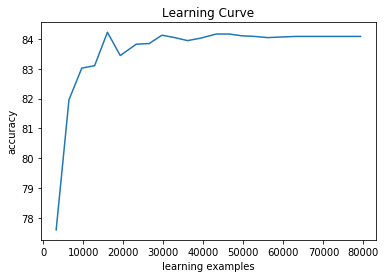
\includegraphics{learning_curve.png}

all code can be found at https://github.com/haoNTT 
%----------------------------------------------------------------------------------------
%	PROBLEM 1
%----------------------------------------------------------------------------------------

\section*{Results} % Numbered section

The hyper-parameters tested in this programs are: 

1. Different tokenization schemes: basic tokenization and advanced tokenization

2. N-gram tokenizations: N ranges from 1 to 4

3. Vocabulary sizes 

4.Embedding dimensions 

5.Learning rate: different choices of values or weather the annealing is applied

6.Optimizer: Adam optimizer or SGD optimizer
%----------------------------------------------------------------------------------------
%	PROBLEM 2
%----------------------------------------------------------------------------------------

\section{Results}

\begin{table}[ht]
\caption{Basic 1-gram Tokenization Result Table} 
\begin{tabular}{c c c c c c} % centered columns (4 columns)
\hline\hline %inserts double horizontal lines
Vocabulary Size & Embedding Dimensions & Optimizer & Learning Rate & Learning Annealing & Accuracy \\ 
\hline 
      15k & 100 & ADAM & 0.01 & No & 0.8356\\
      15k & 200 & ADAM & 0.01 & No & 0.828\\
      15k & 100 & SGD & 0.01 & No & 0.6248\\
      15k & 200 & SGD & 0.01 & No & 0.6642\\
      20k & 100 & ADAM & 0.01 & No & 0.8314\\
      20k & 200 & ADAM & 0.01 & No & 0.8288\\
      15k & 100 & ADAM & 0.01 & Yes & 0.8476\\
      15k & 100 & ADAM & 0.03 & Yes & 0.8432\\
      15k & 100 & ADAM & 0.1 & Yes & 0.8354\\ 
\hline %inserts single line
\end{tabular}
\label{table:nonlin} % is used to refer this table in the text
\end{table}

\begin{table}[ht]
\caption{Basic 2-gram Tokenization Result Table} 
\begin{tabular}{c c c c c c} % centered columns (4 columns)
\hline\hline %inserts double horizontal lines
Vocabulary Size & Embedding Dimensions & Optimizer & Learning Rate & Learning Annealing & Accuracy \\ 
\hline 
      15k & 100 & ADAM & 0.01 & No & 0.817\\
      15k & 200 & ADAM & 0.01 & No & 0.8222\\
      15k & 300 & ADAM & 0.01 & No & 0.819\\
      15k & 100 & SGD & 0.01 & No & 0.506\\
      20k & 100 & ADAM & 0.01 & No & 0.8356\\
      20k & 200 & ADAM & 0.01 & No & 0.8228\\
      20k & 100 & SGD & 0.01 & No & 0.5642\\
      20k & 100 & ADAM & 0.01 & Yes & 0.8412\\
      20k & 100 & ADAM & 0.03 & Yes & 0.8329\\
\hline %inserts single line
\end{tabular}
\label{table:nonlin} % is used to refer this table in the text
\end{table}

\begin{table}[ht]
\caption{Basic 3-gram Tokenization Result Table} 
\begin{tabular}{c c c c c c} % centered columns (4 columns)
\hline\hline %inserts double horizontal lines
Vocabulary Size & Embedding Dimensions & Optimizer & Learning Rate & Learning Annealing & Accuracy \\ 
\hline 
      15k & 100 & ADAM & 0.01 & No & 0.817\\
      15k & 200 & ADAM & 0.01 & No & 0.8222\\
      15k & 100 & SGD & 0.01 & No & 0.521\\
      15k & 200 & SGD & 0.01 & No & 0.554\\
      20k & 100 & ADAM & 0.01 & No & 0.8286\\
      20k & 200 & ADAM & 0.01 & No & 0.8228\\
      20k & 100 & ADAM & 0.01 & Yes & 0.839\\
      20k & 100 & ADAM & 0.03 & Yes & 0.8298\\
\hline %inserts single line
\end{tabular}
\label{table:nonlin} % is used to refer this table in the text
\end{table}

\begin{table}[ht]
\caption{Basic 4-gram Tokenization Result Table} 
\begin{tabular}{c c c c c c} % centered columns (4 columns)
\hline\hline %inserts double horizontal lines
Vocabulary Size & Embedding Dimensions & Optimizer & Learning Rate & Learning Annealing & Accuracy \\ 
\hline 
      15k & 100 & ADAM & 0.01 & Yes & 0.7222\\
      15k & 100 & ADAM & 0.01 & No & 0.728\\
      15k & 100 & SGD & 0.01 & Yes & 0.5016\\
      15k & 100 & SGD & 0.01 & No & 0.4998\\
      20k & 100 & ADAM & 0.01 & Yes & 0.7252\\
      20k & 100 & ADAM & 0.01 & No & 0.7268\\
      20k & 100 & ADAM & 0.03 & Yes & 0.7374\\
\hline %inserts single line
\end{tabular}
\label{table:nonlin} % is used to refer this table in the text
\end{table}

\begin{table}[ht]
\caption{Advanced 1-gram Tokenization Result Table} 
\begin{tabular}{c c c c c c} % centered columns (4 columns)
\hline\hline %inserts double horizontal lines
Vocabulary Size & Embedding Dimensions & Optimizer & Learning Rate & Learning Annealing & Accuracy \\ 
\hline 
      15k & 100 & ADAM & 0.01 & Yes & 0.8422\\
      20k & 100 & ADAM & 0.01 & No & 0.7918\\
      20k & 100 & ADAM & 0.01 & Yes & 0.843\\
      20k & 200 & ADAM & 0.01 & Yes & 0.843\\
      20k & 100 & ADAM & 0.1 & Yes & 0.8222\\
      20k & 200 & SGD & 0.01 & Yes & 0.5208\\
\hline %inserts single line
\end{tabular}
\label{table:nonlin} % is used to refer this table in the text
\end{table}

\begin{table}[ht]
\caption{Advanced 2-gram Tokenization Result Table} 
\begin{tabular}{c c c c c c} % centered columns (4 columns)
\hline\hline %inserts double horizontal lines
Vocabulary Size & Embedding Dimensions & Optimizer & Learning Rate & Learning Annealing & Accuracy \\ 
\hline 
      15k & 100 & ADAM & 0.01 & Yes & 0.8168\\
      20k & 100 & ADAM & 0.01 & No & 0.8152\\
      20k & 100 & ADAM & 0.01 & Yes & 0.8246\\
      20k & 200 & ADAM & 0.01 & Yes & 0.8188\\
      20k & 100 & ADAM & 0.1 & Yes & 0.812\\
      20k & 200 & SGD & 0.01 & Yes & 0.5128\\
\hline %inserts single line
\end{tabular}
\label{table:nonlin} % is used to refer this table in the text
\end{table}

\begin{table}[ht]
\caption{Advanced 3-gram Tokenization Result Table} 
\begin{tabular}{c c c c c c} % centered columns (4 columns)
\hline\hline %inserts double horizontal lines
Vocabulary Size & Embedding Dimensions & Optimizer & Learning Rate & Learning Annealing & Accuracy \\ 
\hline 
      15k & 100 & ADAM & 0.01 & Yes & 0.7631\\
      20k & 100 & ADAM & 0.01 & No & 0.7346\\
      20k & 100 & ADAM & 0.01 & Yes & 0.786\\
      20k & 200 & ADAM & 0.01 & Yes & 0.7722\\
      20k & 200 & SGD & 0.01 & Yes & 0.514\\
\hline %inserts single line
\end{tabular}
\label{table:nonlin} % is used to refer this table in the text
\end{table}

\begin{table}[ht]
\caption{Advanced 4-gram Tokenization Result Table} 
\begin{tabular}{c c c c c c} % centered columns (4 columns)
\hline\hline %inserts double horizontal lines
Vocabulary Size & Embedding Dimensions & Optimizer & Learning Rate & Learning Annealing & Accuracy \\ 
\hline 
      20k & 100 & ADAM & 0.01 & Yes & 0.742\\
      20k & 300 & ADAM & 0.01 & Yes & 0.7512\\
\hline %inserts single line
\end{tabular}
\label{table:nonlin} % is used to refer this table in the text
\end{table}

\begin{table}[ht]
\caption{1-gram Tokenization for Score Rating Result Table} 
\begin{tabular}{c c c c c c} % centered columns (4 columns)
\hline\hline %inserts double horizontal lines
Vocabulary Size & Embedding Dimensions & Optimizer & Learning Rate & Learning Annealing & Accuracy \\ 
\hline 
      30k & 100 & ADAM & 0.01 & Yes & 0.4028\\
      30k & 200 & ADAM & 0.01 & Yes & 0.3960\\
\hline %inserts single line
\end{tabular}
\label{table:nonlin} % is used to refer this table in the text
\end{table}


\end{document}
